\documentclass[fleqn]{beamer}

\usepackage[british]{babel}
\usepackage{graphicx,ru,url}
\usepackage{amsmath}
% Use Times for math font and text font.
\RequirePackage[T1]{fontenc}
%\RequirePackage{txfonts}
% bold math must be loaded after Times font
\usepackage{bm}
\usepackage{booktabs} % nice rules (thick lines) for tables
\usepackage{microtype} % improves typography for PDF
\usepackage{xcolor} % Allows colors in fonts
\usepackage{tikz} % Allows creation of tikz pictures
\usepackage{verbatim}
\usetikzlibrary{arrows,shapes,snakes}
\usepackage{hyperref}
% \usepackage{minted} % Allows printing of python (or other) code
% \newminted{python}{fontsize=\scriptsize, 
%     linenos,
%     numbersep=8pt,
%     gobble=4,
%     frame=lines,
%     bgcolor=bg,
%     framesep=3mm}

% The title of the presentation:
%  - first a short version which is visible at the bottom of each slide;
%  - second the full title shown on the title slide;
\title[Trelis Tutorial]{
    Trelis Tutorial}

% Optional: a subtitle to be displayed on the title slide
%\subtitle{Show where you're from}

% The author(s) of the presentation:
%  - again first a short version to be displayed at the bottom;
%  - next the full list of authors, which may include contact information;
\author[Ye Cheng]{
    Ye Cheng}

% The institute:
%  - to start the name of the university as displayed on the top of each slide
%    this can be adjusted such that you can also create a Dutch version
%  - next the institute information as displayed on the title slide
\institute[Kansas State University]{
    Mechanical and Nuclear Engineering \\
    Kansas State University}

% Add a date and possibly the name of the event to the slides
%  - again first a short version to be shown at the bottom of each slide
%  - second the full date and event name for the title slide
\date[CORPS-G]{
    CORPS-G Group Meeting \\
    02/22/2019}

\begin{document}
    % These two commands allow bonus slides at the end
    % The bonus slides will not be numbered
    \newcommand{\beginbackup}{
        \newcounter{framenumbervorappendix}
        \setcounter{framenumbervorappendix}{\value{framenumber}}
    }
    \newcommand{\backupend}{
        \addtocounter{framenumbervorappendix}{-\value{framenumber}}
        \addtocounter{framenumber}{\value{framenumbervorappendix}} 
    }
    
    \begin{frame}
        \titlepage
    \end{frame}
%%%%%%%%%%%%%%%%%%%%%%%%%%%%%%%%%%%%%%%%%%%%%%%%%%%%%%%%%%%%%%%%%%%%%%%%%%%  
% Outline
    \begin{frame}
        \frametitle{Outline}
        \begin{block}{Presentation Outline}
            \begin{itemize}
                \item Installation
                \begin{itemize}
                    \item Trelis installation
                    \item MCNP plugin installation
                \end{itemize}
                \item Simple meshing instruction
                \begin{itemize}
                 \item Trelis syntax
                 \item Python in Trelis
                \end{itemize}
                \item Meshing
                \item Decomposition
                \item examples
		  \begin{itemize}
		   \item single pin element meshing
		   \item UWNR bare core meshing
		  \end{itemize}

            \end{itemize}
        \end{block}
    \end{frame}
%%%%%%%%%%%%%%%%%%%%%%%%%%%%%%%%%%%%%%%%%%%%%%%%%%%%%%%%%%%%%%%%%%%%%%%%%%%    
\section{Installation}
\begin{frame}
 \frametitle{Install Trelis}
 \begin{itemize}
 \item Request Trelis Trial or license on \textbf{www.csimsoft.com}.
 \item The latest Trelis version is 16.3.5.
 \item Install the Trelis package on your machine.
  \end{itemize}
\end{frame}

\begin{frame}
\frametitle{Install Trelis mcnp-plugin}
\begin{block}{What is Trelis mcnp-plugin}
\begin{itemize}
 \item MCNP2CAD  is a program developed by CNERG from University of Wisconsin to extract the geomtery from MCNP input files and write it out
to a Trelis/Cubit CAD file.
 \item The workflow is: MCNP6 script $\rightarrow$ Trelis MCNP2CAD plugin $\rightarrow$ Trelis CAD file $\rightarrow$ Trelis meshing $\rightarrow$ Further transport code model(Proteus, Rattlesnake, Mammoth, etc). 
\end{itemize}
\end{block}
\end{frame}

\begin{frame}
\frametitle{Install Trelis mcnp-plugin(Cont.)}
\begin{itemize}
\item Download from MCNP2CAD Github repo: \textbf{https://github.com/svalinn/mcnp2cad}. Alternatively, follow the instruction in \textbf{installation\_guide/Trelis\_installation\_instruction}.
 \item There could be package dependency problems causing the mcnp-plugin not able to be loaded. Typically there should be two:
 \begin{itemize}
  \item  \textbf{libMOAB.so.0} is not found because that the \textbf{LD\_LIBRARY\_PATH} has not been set in new user's \textbf{bashrc} file
  \item textbf{libarmadillo.so.6} is not found because the package \textbf{libarmadillo-dev}, on which Trelis-plugins have a dependence, has not been
   installed on new user's computer
 \end{itemize}

The detailed Trelis-fixing instruction can be found in \textbf{installation\_guide/fixing\_mcnp2cad}.
\end{itemize}
\end{frame}
%%%%%%%%%%%%%%%%%%%%%%%%%%%%%%%%%%%%%%%%%%%%%%%%%%%%%%%%%%%%%%%%%%%%%%%%%%%  
\section{Simple meshing instruction}
\begin{frame}
        \frametitle{Trelis GUI window}
        \begin{center}
            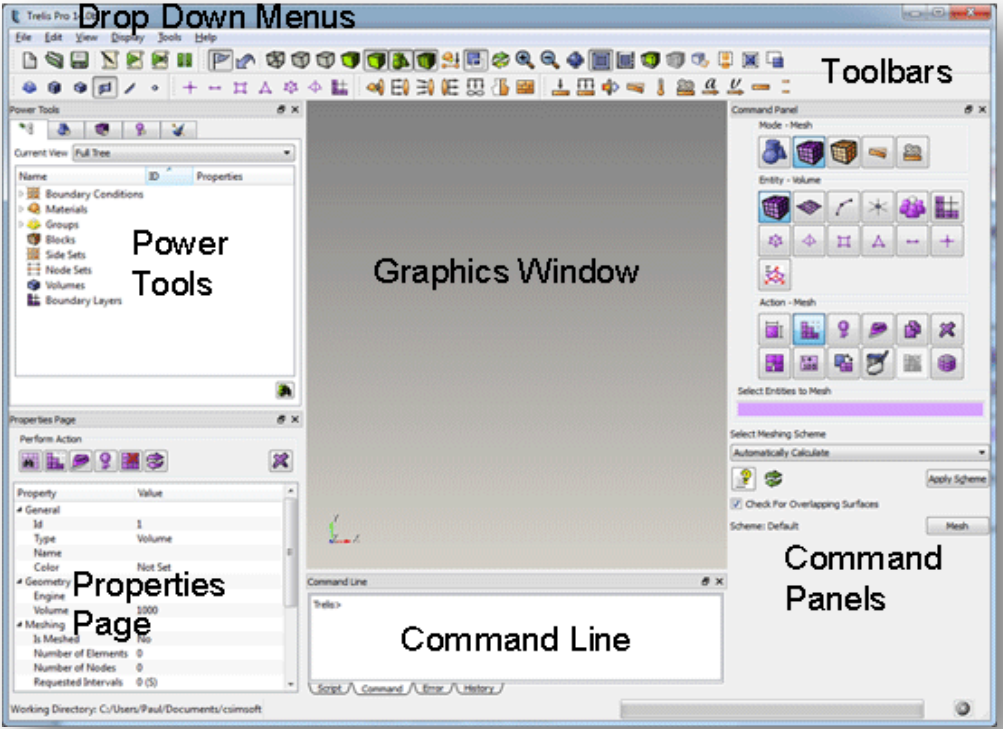
\includegraphics[trim=.1cm .25cm 2.0cm .4cm, clip=true, totalheight=.8\textheight]{figures/gui_window.png}
        \end{center}
\end{frame}

\begin{frame}
\frametitle{Create a simple mesh}
\begin{itemize}
 \item Creating the geometry
 \item Setting the interval sizes and meshing schemes
 \item Meshing the geometry
 \item Specifying the boundary conditions
 \item Exporting the mesh
\end{itemize}
\end{frame}

\begin{frame}
 \frametitle{Generated mesh for brick with cylindrical Hole}
 \begin{itemize}
  \item Step 1: Beginning Execution
  \item Step 2: Creating the Brick
  \item Step 3: Creating the Cylinder
  \item Step 4: Adjusting the Graphics Display
  \item Step 5: Forming the Hole
  \item Step 6: Setting Interval Sizes
  \item Step 7: Surface Meshing
  \item Step 8: Volume Meshing
  \item Step 9: Inspecting the Model
  \item Step 10: Materials and Boundary Conditions
  \item Step 11: Exporting the Mesh
 \end{itemize}
\end{frame}

\begin{frame}
 \frametitle{Generated mesh for brick with cylindrical Hole(Cont.)}

\begin{columns}[t]
\column{.33\textwidth}
\centering
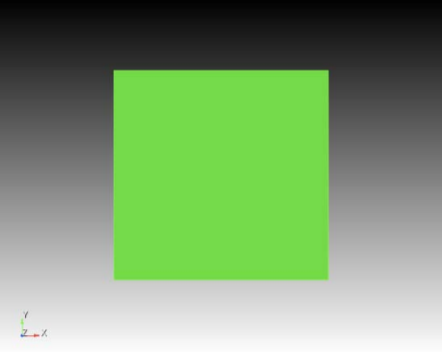
\includegraphics[width=3cm,height=2cm]{figures/step_2.png}\\
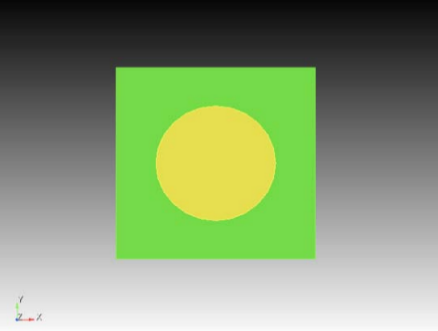
\includegraphics[width=3cm,height=2cm]{figures/step_3.png}\\
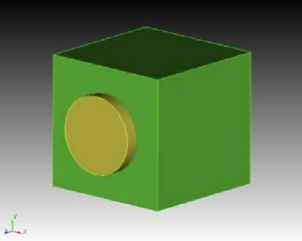
\includegraphics[width=3cm,height=2cm]{figures/step_4.png}
\column{.33\textwidth}
\centering
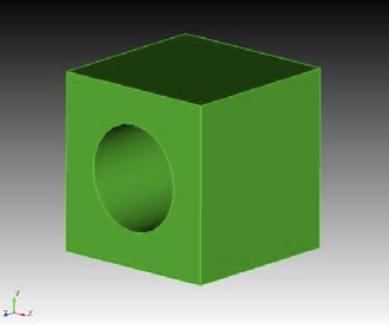
\includegraphics[width=3cm,height=2cm]{figures/step_5.png}\\
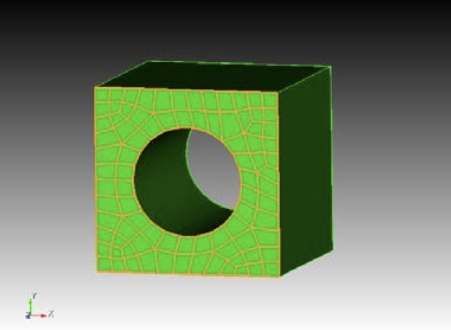
\includegraphics[width=3cm,height=2cm]{figures/step_7.png}\\
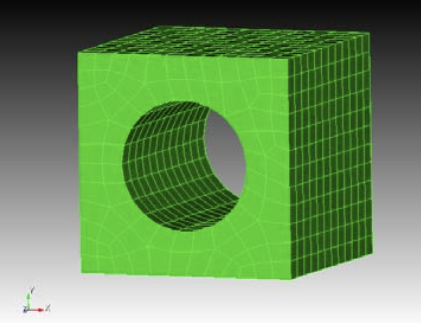
\includegraphics[width=3cm,height=2cm]{figures/step_8.png}\\
\column{.33\textwidth}
\centering
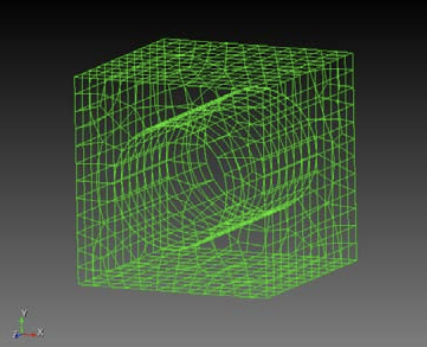
\includegraphics[width=3cm,height=2cm]{figures/step_9.png}\\
\end{columns}

\end{frame}














%%%%%%%%%%%%%%%%%%%%%%%%%%%%%%%%%%%%%%%%%%%%%%%%%%%%%%%%%%%%%%%%%%%%%%%%%%%










%%%%%%%%%%%%%%%%%%%%%%%%%%%%%%%%%%%%%%%%%%%%%%%%%%%%%%%%%%%%%%%%%%%%%%%%%%%

    \section{Section 1}
    
    \begin{frame}
        \frametitle{Title of the Slide}
        Here is some Slide content.
        
        You can do many things with the slides.
        
        Over the next couple slides I will demonstrate some different kinds of slides.
    \end{frame}
    
    \section{Different Slides} % new section title
    \begin{frame}
        \frametitle{Column Slide}
        This is how to make a 2 column slide
        \begin{columns}[c]
            \begin{column}{0.5\textwidth} % split the columns 50/50
                \begin{block}{Block Title}
                    \begin{itemize}
                        \item Some list of things
                        \item More things
                    \end{itemize}
                \end{block}
            \end{column}
            
            \begin{column}{0.5\textwidth} % Other half of the column split
                Here is an equation
                \begin{equation}
                    \mathcal{T} \phi(\bm{\rho}) = \frac{1}{k} \mathcal{F} \phi(\bm{\rho}) \, , \nonumber
                \end{equation}
                where $\bm{\rho}$ contains the relevant phase space (i.e., $\mathbf{r}$, $E$, and $\Omega$).
            \end{column}
        \end{columns}
    \end{frame}
    
    \begin{frame} % This is a slide with a picture created by tikz
        \frametitle{Picture Slide}
        \begin{block}{Pin Cell Mesh}
            \begin{itemize}
                \item 22 mesh cells of fuel 
                \item 3 mesh cells of moderator on either side
                \item Each pin cell provides 28 energy-dependent snapshots
            \end{itemize}
        \end{block}
        \begin{center}
            \begin{figure} % Here you can use any figure
                % Now create a figure with tikz
                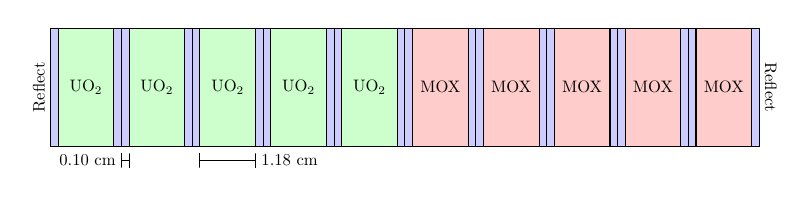
\begin{tikzpicture}[scale=0.6, every node/.style={scale=0.6}]
                    \foreach \x in {0,1.5,...,6}
                    \filldraw[xshift=\x cm, fill=green!20!white, draw=black] (0.160714286,0) rectangle (1.339285714,2.5) node[pos=.5] {UO$_2$};
                    \foreach \x in {7.5,9,...,13.5}
                    \filldraw[xshift=\x cm, fill=red!20!white, draw=black] (0.160714286,0) rectangle (1.339285714,2.5) node[pos=.5] {MOX};
                    \foreach \x in {0,1.5,...,13.5}
                    \filldraw[xshift=\x cm, fill=blue!20!white, draw=black] (0,0) rectangle (0.160714286,2.5);
                    \foreach \x in {0,1.5,...,13.5}
                    \filldraw[xshift=\x cm, fill=blue!20!white, draw=black] (1.339285714,0) rectangle (1.5,2.5);
                    \draw[xshift=15cm,yshift=1.25cm] node[right] {\rotatebox{-90}{Reflect}};
                    \draw[yshift=1.25cm] node[left] {\rotatebox{90}{Reflect}};
                    \draw (1.5,-.15) -- (1.5,-.45) -- (1.5,-.30) node[left] {0.10 cm} -- (1.660714286,-.30) -- (1.660714286,-.15) -- (1.660714286, -.45);
                    \draw (3.160714286,-.15) -- (3.160714286,-.45) -- (3.160714286,-.30) -- (4.339285714,-.30) node[right] {1.18 cm} -- (4.339285714,-.15) -- (4.339285714, -.45);
                \end{tikzpicture}
            \end{figure}
        \end{center}
        \begin{block}{Test Problem Settings}
            \begin{itemize}
                \item 16-angle, double Gauss-Legendre quadrature
                \item Step characteristics spatial discretization
            \end{itemize}
        \end{block}
    \end{frame}
    
    \begin{frame}
        % This is a frame with a table in it
        \frametitle{Table Slide}
        \begin{table}
            \begin{tabular}{l | p{7cm}}\toprule
                Abbreviation    & Model to generate snapshots \\ 
                \hline
                MOX Pin         & MOX pin only \\
                UO$_2$ Pin      & UO$_2$ pin only \\
                Combined Pins  & 1 UO$_2$ pin, 1 MOX pin, Pin Junction modeled separately then combined \\
                N pin           & Repeating array of N UO$_2$ and N MOX pin \\
                \bottomrule
            \end{tabular}
            \label{tab:snapshots}
        \end{table}
    \end{frame}
    
    \begin{frame}
        \frametitle{Frame with Blocks}
        \begin{block}{The Karhunen Lo\'{e}ve Transform :}
            \begin{itemize}
                \item Shows improvement over mDLP
                \item Reduces DOF needed for accurate results
                \item Generally improves with increased information
                \item Achieves sub $0.1\%$ error with $<1/10$ DOF
            \end{itemize}
        \end{block}
        \begin{block}{Future Work}
            \begin{itemize}
                \item Expanding to 2D
                \item KLT on spatial variable
                \item Test basis functions using 1 group of snapshots
            \end{itemize}
        \end{block}
        \begin{block}{Contact Information}
            \begin{itemize}
                \item Your Name: Your email
                \item Dr. Jeremy Roberts: jaroberts@k-state.edu
            \end{itemize}
        \end{block}
        
        % This line allows a reference slide without citing references
        \nocite{*}
    \end{frame}
    
%     \defverbatim[colored]\helloworld{
%         \begin{pythoncode}
%             
%             # We will make our first program!
%             print 'Hello World!'
%             
%             
%         \end{pythoncode}
%     }
%     \begin{frame}
%         \frametitle{Your First Program}
%         In programming some version of this is often the first program
%         \helloworld
%         This will print the string: 
%         
%         Hello World!
%     \end{frame}
    
    \section{References}
    
    \begin{frame}[t,allowframebreaks]\label{lastframe}
        \frametitle{References}
        \bibliographystyle{ans}
        % make a bibliography.bib file with your references in it
        \bibliography{bibliography}
    \end{frame}
    
    \beginbackup % begins the non-numbered slides
    
    \begin{frame}[noframenumbering]
        \frametitle{no frame number slide}
        \begin{center}
            Some words and test figure
            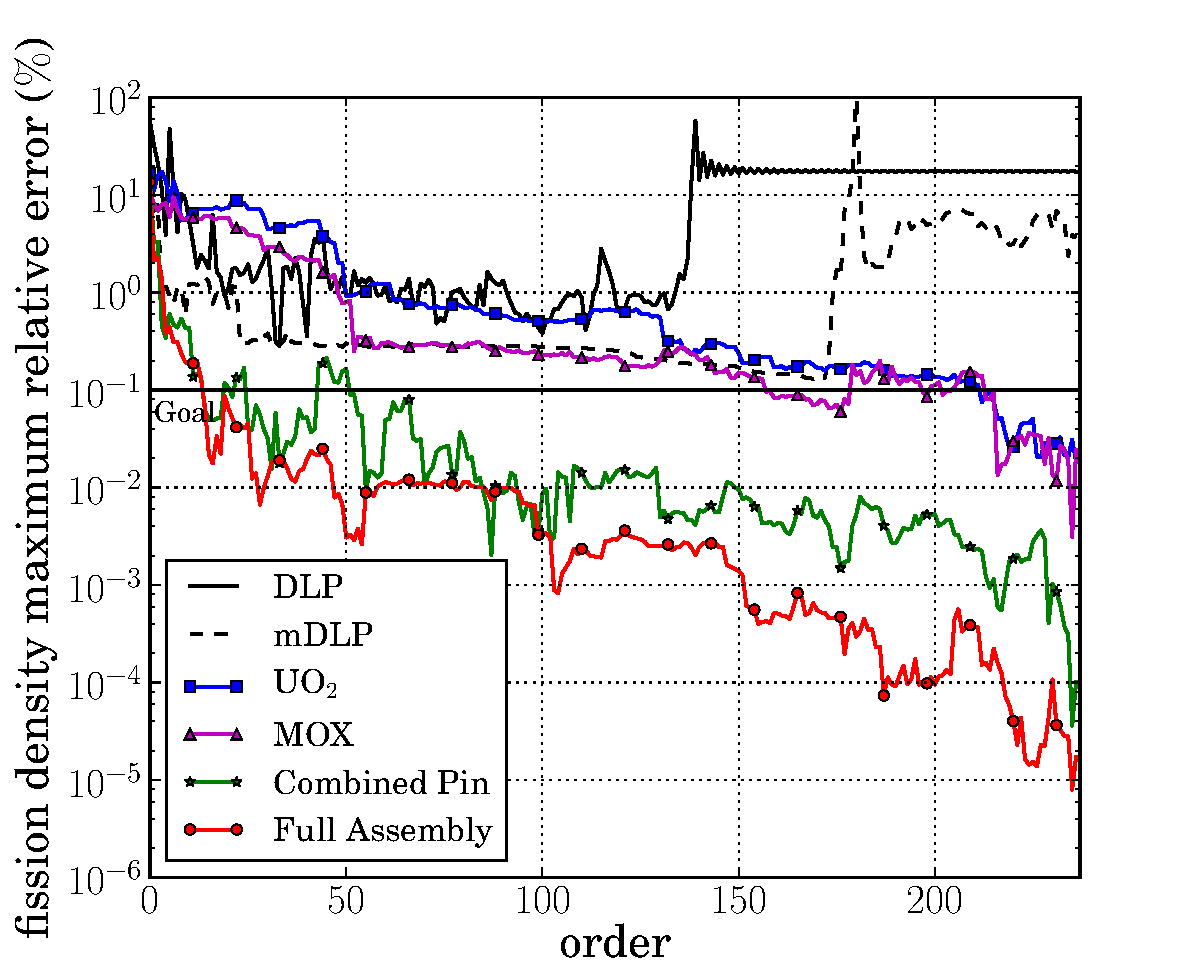
\includegraphics[trim=.1cm .25cm 2.0cm .4cm, clip=true, totalheight=.8\textheight]{sample_figure}
        \end{center}
    \end{frame}
    
    \backupend % Ends the non-numbered slides
    
\end{document}
